\documentclass[12pt, a4paper]{article}

\usepackage[top=2.5cm, bottom=2.5cm, left=3cm, right=2.5cm]{geometry}
\usepackage{graphicx}
\usepackage{float}
\usepackage[hidelinks]{hyperref}
\usepackage{titlesec}
\usepackage{setspace}
\usepackage{lmodern}
\usepackage[T1]{fontenc}
\usepackage[utf8]{inputenc}
\usepackage{indentfirst}
\usepackage{tikz}

\setlength{\parindent}{1.5em}
\setlength{\parskip}{0.7em}

\onehalfspacing

\titleformat{\section}{\large\bfseries}{Chapter \thesection.}{0.5em}{}
\titleformat{\subsection}{\normalsize\bfseries}{\thesubsection.}{0.5em}{}

\begin{document}

% ==============================================================
% Title page — copied from pagedegarde.tex
% ==============================================================
\begin{titlepage}
\singlespacing
	\thispagestyle{empty}
	\newcommand\framethispage[1][1cm]{%
        \begin{tikzpicture}[remember picture,overlay]
        \draw[
            line width=2.5pt
        ]
        ([xshift=#1,yshift=-#1]current page.north west)
        rectangle
        ([xshift=-#1,yshift=#1]current page.south east);
        \end{tikzpicture}%
        }

   	
\includegraphics[width=0.13\textwidth,height=0.14\textwidth]{./USTHB_Logo}
   	\textsc{\normalsize République Algérienne Démocratique et Populaire}
   	
\includegraphics[width=0.13\textwidth,height=0.14\textwidth]{./USTHB_Logo}\\[0.2cm]

   \begin{center}
   	\textbf{\normalsize Ministère de  l'Enseignement Supérieur et de la Recherche Scientifique}\\[0.4cm]

   	\textsc{\normalsize Université des Sciences et de la Technologie Houari Boumediene}\\[0.4cm]

   	\textbf{\normalsize Faculté et d'Informatique}\\[0.3cm]
   	\textbf{\large Département SIQ}\\[0.4cm]
   	\textsc{\normalsize Summary}\\[0.4cm]

   	\textbf{\large Speciality}\\[0.4cm]

   	\textsc{\normalsize Réseau Et Systèmes Distribués}\\[0.4cm]

   \underline{\textbf{\large Subject}}\\[0.2cm]
   \begin{center}
   \setlength{\fboxsep}{3mm}
   \setlength{\fboxrule}{0.8mm}
    \fbox{
         \begin{minipage}{0.85\textwidth}

         \centering \textbf {\large
Conception and Deployment\\[0.05cm] of an Open-Source\\[0.05cm]
Hyper-Converged Private Cloud Infrastructure\\[0.05cm]
}
         \end{minipage}
         }
     \end{center}
   \end{center}

   \vfill

\begin{minipage}{0.4\textwidth}
	\begin{flushleft}
		\normalfont{\textbf{\normalsize Proposé et Dirigé par : }} \\[0.2cm]
		 \normalfont{\textbf{\normalsize   Mr. Neffah Mohammed  }} \\[0.2cm]
		 \normalfont{\textbf{\normalsize   Prof. MERAZKA Fatiha  }} \\[0.4cm]
	\end{flushleft}
\end{minipage}

 \vfill

 \begin{minipage}{0.95\textwidth}
 	\begin{flushright}
 	 \normalfont{\textbf{\normalsize  Réalisé et présenté par :  }} \\[0.2cm]
 	 \normalfont{\textbf{\normalsize  Mr. Bouzara Zakaria}}\\[0.2cm]
 	 \normalfont{\textbf{\normalsize  Mr. Ouacherine Ilyes}} \\[0.4cm]
 	\end{flushright}
 \end{minipage}
 \vfill
\begin{minipage}{0.4\textwidth}
	\begin{flushleft}
		\normalfont{\textbf{\normalsize  Devant le jury composé de : }} \\[0.2cm]
		\normalfont{\textbf{\normalsize  M ........... ........}}\\[0.2cm]
		\normalfont{\textbf{\normalsize  M ........... ........}}\\[0.4cm]
	\end{flushleft}
\end{minipage}

\vfill
	\begin{center}
		\normalfont{\textbf{\normalsize Soutenu le :  ../../2026  }} \\[0.2cm]
		\normalfont{\textbf{\normalsize   Binôme N°  18/2026 }}\\
	\end{center}

\end{titlepage}

\setcounter{page}{0}
\tableofcontents
\newpage

% ==============================================================
\section*{Introduction}
\addcontentsline{toc}{section}{Introduction}
% ==============================================================

Modern enterprise IT infrastructure relies on three fundamental pillars: computing, storage, and networking. For years, each of these was handled by separate, specialized equipment, which made administration complex and expensive. Hyper-Converged Infrastructure (HCI) brings all three layers together on standard servers managed by a centralized software layer, making the whole system simpler to run and easier to scale.

Sonatrach, Algeria's national hydrocarbons company, runs a hyper-converged production environment built on proprietary solutions, mainly Nutanix and VMware vSAN. These platforms are solid, but they come with high licensing costs and a level of vendor dependency that limits the company's technical freedom. For smaller environments, such as test and development clusters, deploying those same solutions is simply disproportionate.

This project asked whether a fully open-source hyper-converged platform could provide the same kind of reliability and performance, at zero licensing cost, on existing hardware. The answer was a three-node private cloud cluster built on Dell PowerEdge R720 servers, combining Proxmox VE, Ceph, and Open vSwitch. The project also produced a custom dynamic load balancing service called CSLB, written in Go, to fill a gap that Proxmox does not address natively.

% ==============================================================
\section{Context, Problematic, and Objectives}
% ==============================================================

\subsection{Sonatrach and Its Infrastructure}

Sonatrach was founded in 1963 and has grown into Africa's largest hydrocarbons company. It covers the entire oil and gas value chain, from exploration and production to transformation and commercialization, and operates in partnership with many international companies. This project was carried out within the Innovation Centre, which belongs to the Directorate of Infrastructure and IT Services, itself part of the Central Directorate of Digitalization and Information Systems (DC DSI).

The company's production infrastructure relies on two proprietary HCI solutions. Nutanix is deployed at scale across multiple sites for critical production workloads, while VMware vSAN is used for smaller deployments. Both platforms are mature and well-supported, but they present constraints that are increasingly problematic over time.

Licensing costs grow every year, regardless of actual usage. The exclusive reliance on these vendors creates a lock-in situation that limits negotiating power and makes it difficult to adapt the infrastructure to the company's specific needs. From a sovereignty standpoint, every architectural decision depends on the vendor's roadmap. For three- or four-node clusters serving test and development environments, these solutions are simply oversized in both complexity and cost.

\subsection{Problematic}

The central question this project addresses is the following: how can a fully open-source hyper-converged private cloud be designed and deployed on existing hardware, while meeting the reliability, performance, and scalability requirements of a large industrial company?

This raises several concrete technical questions. How do you build a distributed storage system that keeps data safe when a node fails? How do you automate the failover and load redistribution of virtual machines across a cluster without service interruption? How do you isolate different network traffic types within the same physical infrastructure? And can an open-source stack realistically compete with proprietary solutions at this scale?

\subsection{Objectives}

The general objective is to design and deploy a fully open-source hyper-converged private cloud on three Dell PowerEdge R720 servers provided by Sonatrach, with reliability and scalability comparable to proprietary solutions.

Several specific objectives support this goal. The first is to deploy a three-node Proxmox VE cluster with centralized management, live migration support, and automatic failover. The second is to configure a Ceph distributed storage cluster using four disks per node as storage daemons, for a total of twelve OSDs, with a replication factor of three. The third is to implement an advanced network segmentation architecture using Open vSwitch and VXLAN tunnels, separating management, replication, migration, and application traffic. The fourth is to develop a dynamic load balancing mechanism capable of automatically redistributing virtual machines based on real-time resource metrics. The fifth is to validate the platform with a high availability scenario. Finally, the project must deliver a documented infrastructure base that Sonatrach can reuse and scale up.

The scope is limited to a test and development environment. The cluster operates on three Dell R720 servers, and the per-node storage capacity is appropriate for development and validation but not for large-scale production data. The physical switch configuration was also outside the project's control, which shaped the network design decisions.

% ==============================================================
\section{Technical Background and Solution Overview}
% ==============================================================

\subsection{Hyper-Converged Infrastructure}

Hyper-converged infrastructure combines computing, storage, and networking into a single layer managed by software. Unlike traditional architectures where each layer requires dedicated hardware, HCI runs everything on standard servers. This brings simpler administration through a unified interface, lower hardware costs by eliminating dedicated storage arrays, horizontal scalability by adding nodes, and native high availability through data replication across nodes.

\subsection{Technologies Chosen}

Three open-source technologies form the core of this infrastructure. Proxmox VE is the hypervisor. It is based on KVM for full virtual machines and LXC for lightweight containers, and runs on a modified Debian Linux kernel. It uses less than 1 GB of RAM when idle, deploys a three-node cluster in a few hours, and integrates Ceph natively. Its REST API on port 8006 exposes all operations programmatically. Cluster membership and quorum are managed by Corosync, which requires a minimum of three nodes to avoid split-brain situations. The built-in HA manager detects node failures and restarts protected virtual machines on surviving nodes within 60 to 120 seconds.

Ceph handles distributed storage. It uses a RADOS core with Monitor, Manager, and OSD daemons. The CRUSH algorithm places data replicas across different physical nodes without a central directory. With replication factor three and twelve OSDs across three nodes, the cluster tolerates the complete loss of one node without any data loss.

Open vSwitch provides software-defined networking. Because the physical switch at Sonatrach was not accessible for VLAN configuration, VXLAN tunnels were used instead. VXLAN encapsulates Ethernet frames inside UDP packets, creating isolated logical networks on top of the existing physical network without modifying it. Each logical network is identified by a unique VXLAN Network Identifier (VNI).

\subsection{Complementary Tools}

Monitoring relies on InfluxDB for time-series metrics from Proxmox, Prometheus for Ceph and CSLB metrics, Grafana for dashboards and alerts, and Loki with Grafana Alloy for centralized log collection. Infrastructure automation uses Ansible playbooks executed over SSH, with GitLab for code versioning and CI/CD pipelines, and Rundeck to expose playbooks through a web interface. OPNsense handles inter-network routing and firewall filtering. Chrony synchronizes time across all nodes, which is critical for both Ceph and Corosync. A PXE and TFTP provisioning pipeline was also designed to automate bare-metal installation of new nodes from power-on to cluster membership.

The CSLB service fills the gap left by Proxmox's lack of a native proactive load balancer, equivalent to VMware's Distributed Resource Scheduler. It is an adaptation of the CSLB algorithm, extended to consider both CPU and RAM, with anti-oscillation protections and a circuit breaker.

% ==============================================================
\section{Architecture and Conception}
% ==============================================================

\subsection{Overall Architecture}

The infrastructure is organized in three layers. The physical layer consists of three Dell PowerEdge R720 servers, each running Proxmox VE installed directly in bare-metal mode. The virtualization and cluster layer groups the three Proxmox nodes, PVE-01, PVE-02, and PVE-03, into a high-availability cluster. Each node simultaneously runs Ceph storage daemons and an Open vSwitch instance, which is the defining characteristic of hyper-convergence. The application and services layer hosts the OPNsense VM, the demo application, the CSLB service, the monitoring stack, and the automation tools.

\begin{figure}[H]
    \centering
    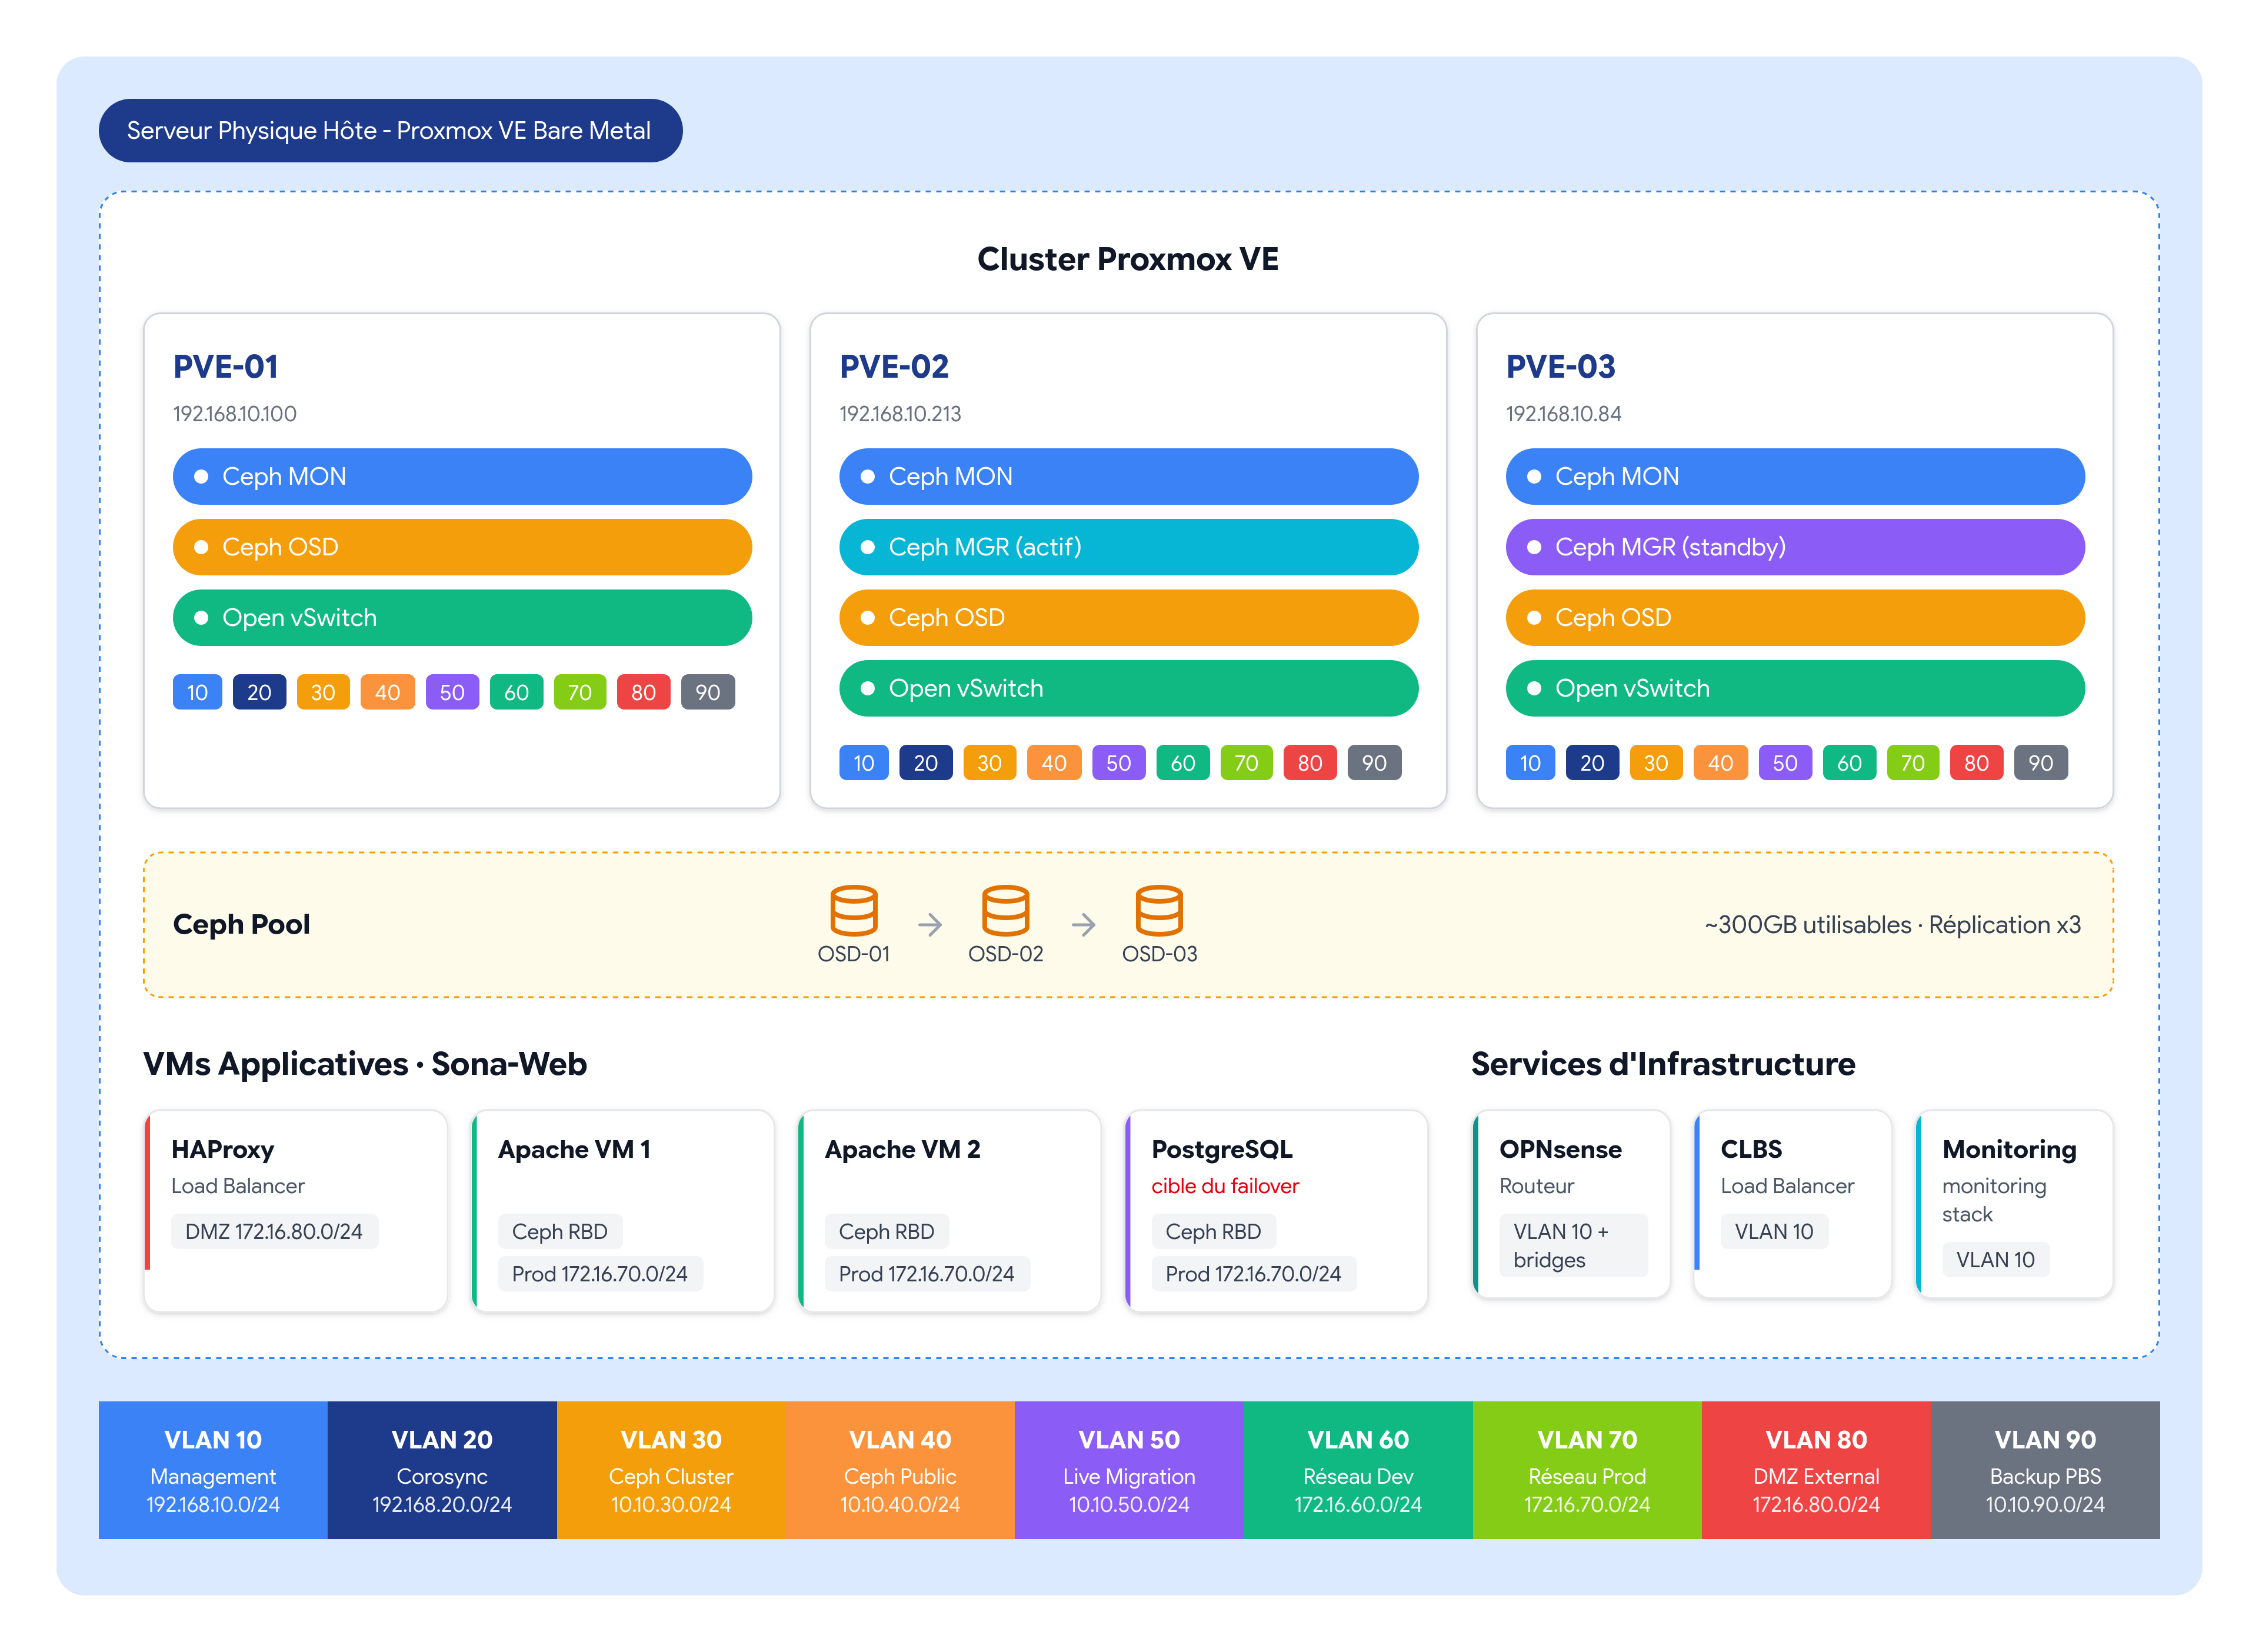
\includegraphics[width=\textwidth]{image/ch3/architecture-hci.jpg}
    \caption{Overall Architecture of the HCI Infrastructure}
    \label{fig:arch-globale}
\end{figure}

Figure~\ref{fig:arch-globale} shows the three superimposed layers of the architecture. The bottom layer contains the physical servers. The middle layer carries Proxmox, Ceph, and Open vSwitch running together on each node. The top layer hosts the services and virtual machines. The design was organized into three interdependent parts: Compute, Storage, and Network.

\subsection{Compute}

Each Dell R720 server has five SAS disks. One 300 GB disk is reserved for the Proxmox operating system. The remaining four disks, one 300 GB and three 600 GB, become Ceph OSDs. PVE-01 has 64 GB of RAM while PVE-02 and PVE-03 each have 254 GB.

The cluster uses Corosync for heartbeat communication on a dedicated VXLAN segment. With three nodes, the quorum requires two active nodes to operate. If one node goes down, the other two maintain the quorum, the HA manager restarts protected virtual machines on surviving nodes, and Ceph continues serving data from its remaining replicas. If two nodes go down simultaneously, the cluster freezes to prevent data corruption.

The CSLB service is one of the main contributions of this project. It runs every 60 seconds, reads 5-minute averaged CPU and RAM metrics from InfluxDB, and computes a moderated band around the cluster average. A node is considered overloaded if its CPU or RAM exceeds the upper boundary of this band and also exceeds 50\% in absolute terms. When a node is overloaded, CSLB selects the best virtual machine to migrate, based on a transfer vector derived from the original CSLB algorithm, and picks the destination node using a weighted score that gives 70\% weight to CPU and 30\% to RAM. The service will not migrate the same VM twice within 10 minutes, and it suspends itself for one hour if more than six migrations happen in 30 minutes. This circuit breaker prevents oscillation storms.

A demo application called Sona-Web was deployed to validate the platform. It consists of four Debian VMs: an HAProxy load balancer, two Flask application instances, and a PostgreSQL database. HAProxy checks backend health every 200 ms and reroutes traffic in under 200 ms if an instance becomes unreachable, which also happens during live migrations.

Monitoring runs in a dedicated LXC container. InfluxDB receives Proxmox node and VM metrics via the native Metric Server mechanism. Prometheus scrapes Ceph cluster metrics from the MGR daemon on port 9283 and CSLB application metrics on port 9101. Grafana connects to both sources and provides unified dashboards covering node load, storage health, migration history, and alerts. Loki, fed by Grafana Alloy agents on each node, centralizes system and firewall logs.

Ansible handles infrastructure automation through four playbooks: VM provisioning from a Debian cloud-init template, bootstrapping new machines with the Ansible user and SSH key, NTP configuration across the cluster, and batch VM creation from a YAML list. A PXE/TFTP provisioning pipeline was fully designed to automate the physical installation of Proxmox on a new server from power-on to cluster membership in under 25 minutes, with no manual input. Its implementation requires dedicated server hardware that was not available during the project, so its validation is left as a perspective.

\subsection{Storage}

The Ceph cluster uses three Monitor daemons, one per node, for cluster map consensus, and two Manager daemons, one active on PVE-02 and one standby on PVE-03, for metrics and management. The twelve OSDs are distributed four per node across disks sdb to sde.

With replication factor three, every data block gets one copy on each physical node. The usable capacity is approximately 2.05 TB. The CRUSH map is configured with host-level failure domains, meaning the three replicas of any block are always placed on three different physical servers. When a node is lost, Ceph marks the affected OSDs as down, the pool enters a degraded state, and data remains accessible via the surviving replicas. After the node is restored, Ceph automatically rebuilds the missing replicas.

\subsection{Network}

The network design had to work around a hard constraint: the physical Sonatrach switch only exposes the native management VLAN and cannot be reconfigured. VXLAN tunnels running over Open vSwitch solve this cleanly. Each node creates point-to-point VXLAN tunnels toward the other two, and each tunnel carries a specific type of traffic identified by its VNI.

Five infrastructure networks handle cluster internal traffic: management (VNI 10), Corosync heartbeat (VNI 20), Ceph internal replication (VNI 30), Ceph public access from VMs (VNI 40), and live migration (VNI 50). Three more VXLANs carry application traffic: Dev (VNI 60), Prod (VNI 70), and DMZ (VNI 80).

OPNsense runs as a VM with four network interfaces: a WAN interface on the management network and three LAN interfaces, one per application zone. It acts as the centralized router and firewall for all application traffic, providing NAT for outbound access and DHCP for each internal network. The firewall enforces zone isolation: Dev cannot reach Prod or DMZ, Prod can only reach DMZ, and direct WAN access from Prod is blocked. A second firewall layer at the Proxmox hypervisor level protects infrastructure networks, blocking any application VM from reaching Corosync or Ceph replication segments, and restricting access to the Proxmox management interface to the management subnet only.

% ==============================================================
\section{Implementation and Results}
% ==============================================================

\subsection{Deployment Approach}

The deployment was carried out directly on the physical servers, using the Proxmox web interface for most operations and the command line for tasks the interface does not cover. There was no pre-existing automation to bootstrap from, so the initial setup was done step by step, node by node, before playbooks took over for repeatable operations.

Proxmox VE was installed from a USB drive on each node, with a static IP assigned on the management network. Once the three nodes were up, the cluster was formed with a single command on PVE-01, and the other two nodes joined by pointing at PVE-01's IP. The Proxmox web interface confirmed the three-node cluster with quorum achieved.

The Ceph cluster was initialized via the \texttt{pveceph} command set. One monitor was created on each node, two managers were deployed on PVE-02 and PVE-03, and then all four data disks on each node were formatted and added as OSDs. The pool was created with replication factor three and a minimum of two required replicas. The result was a healthy cluster with twelve OSDs and roughly 2.05 TB of usable capacity.

The Open vSwitch and VXLAN configuration was written manually into the \texttt{/etc/network/interfaces} file on each node. Each node lists the IP addresses of the other two in its tunnel definitions, which is a requirement of point-to-point VXLAN mode. OPNsense was then deployed as a VM with its four interfaces connected to the appropriate bridges.

\subsection{Services and Automation}

The monitoring stack was deployed in a single LXC container. InfluxDB was configured as the Proxmox Metric Server target, Prometheus scraped the Ceph MGR endpoint after enabling the module, and Grafana was connected to both. Dashboards showing cluster load, storage health, OSD latency, and CSLB migration history were operational quickly.

The CSLB service was written in Go, compiled to a static binary, and deployed on a dedicated VM as a systemd service with automatic restart. Its logs show the classification of nodes into heavy, moderate, and light bands at every 60-second cycle, along with migration events and cooldown periods. A validation test using \texttt{stress-ng} to saturate CPU on two VMs confirmed that CSLB detected the imbalance and triggered a live migration to the least-loaded node, which was visible in the Grafana dashboard.

Four Ansible playbooks were implemented and tested. GitLab CE was deployed as an LXC container and hosts the CSLB source code and the Ansible playbook repository. CI/CD pipelines run linting and unit tests on every push. Rundeck was deployed alongside GitLab and exposes the provisioning playbooks through a web interface.

\subsection{Validation and Results}

The high availability scenario was validated by powering off one node while virtual machines were running. Corosync detected the loss within its heartbeat window, the HA manager triggered the fencing mechanism and restarted protected VMs on the surviving nodes. The Sona-Web application remained accessible throughout. After the node was powered back on, the cluster resynchronized and returned to a fully healthy state.

Live migration was tested both manually through the Proxmox interface and automatically via CSLB. In both cases, the VM transferred without service interruption. The Sona-Web application continued serving requests during migrations, with HAProxy handling the short transition window transparently.

\subsection{What Was Not Implemented}

The PXE and TFTP provisioning pipeline, designed to automate the full installation of Proxmox on a bare physical server from network boot to cluster membership, could not be tested because no spare server hardware was available for the TFTP and HTTP servers during the lab period. Its design is documented in detail in the conception chapter.

The identity management layer also remained simplified. The design included an OpenLDAP directory server to centralize authentication across Proxmox, Grafana, GitLab, and Rundeck. Due to time constraints, the native Proxmox user management system was used instead, and OpenLDAP remains a planned extension.

% ==============================================================
\section*{Conclusion}
\addcontentsline{toc}{section}{Conclusion}
% ==============================================================

This project demonstrated that a fully open-source hyper-converged infrastructure can meet the reliability and operational requirements of a large industrial enterprise. The deployed platform runs on three Dell PowerEdge R720 servers and delivers high availability, distributed storage with triple replication, advanced network segmentation, dynamic load balancing, centralized monitoring, and infrastructure automation, all without any licensing cost.

The main objectives were achieved. The three-node Proxmox cluster formed successfully with Corosync quorum. Ceph deployed twelve OSDs with 2.05 TB of usable storage and withstood a simulated node failure without data loss. The VXLAN segmentation created eight isolated logical networks on top of a single physical link. The CSLB service detected load imbalance and triggered live migrations automatically. The high availability scenario confirmed automatic VM restart after node failure and automatic storage resynchronization after node recovery.

Compared to proprietary solutions, the platform eliminates licensing costs entirely and gives full access to the underlying code, which means Sonatrach can adapt it to its own needs without waiting for vendor updates. Compared to OpenStack, it is far lighter and operational in hours on a three-node cluster. Compared to Harvester, it handles classical Linux and Windows virtual machines more efficiently with a smaller host memory footprint. The development of CSLB also fills a real gap in Proxmox by adding proactive load balancing that the platform does not provide natively.

Several directions can extend the platform further. The PXE and Ansible pipeline should be validated on dedicated hardware to fully automate the integration of new physical nodes. The current VXLAN configuration could be replaced by native OVS VLANs managed through the Proxmox SDN module, provided access to the Sonatrach switch becomes available. Centralizing authentication with OpenLDAP would unify access management across Proxmox, Grafana, GitLab, and Rundeck. Replacing the current alerting stack with Wazuh would add intrusion detection, file integrity monitoring, and event correlation. Finally, deploying Apprise as a notification layer would route alerts to multiple channels without depending on an external SMTP server.

\end{document}
